% This file was created with tikzplotlib v0.10.1.
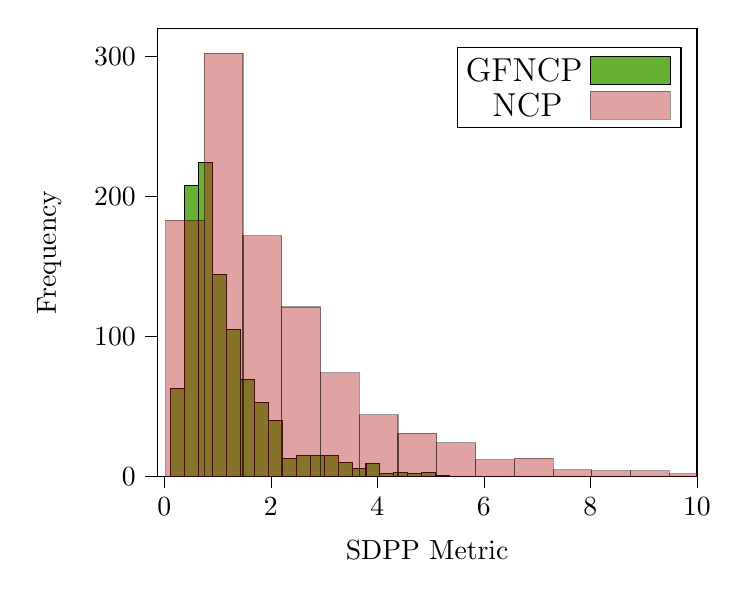
\begin{tikzpicture}

\definecolor{darkgray176}{RGB}{176,176,176}
\definecolor{green_1}{RGB}{173,216,230}
% \definecolor{green_1}{RGB}{173,216,230}
\definecolor{green_1}{rgb}{0.6, 0.81, 0.93}
\definecolor{forestgreen4416044}{RGB}{44,160,44}
\definecolor{red_1}{RGB}{178,24,24}
\definecolor{green_1}{rgb}{0.4, 0.69, 0.2}

\begin{axis}[
tick align=outside,
tick pos=left,
x grid style={darkgray176},
xlabel={SDPP Metric},
xmin=-0.13, xmax=10,
xtick style={color=black},
y grid style={darkgray176},
ylabel={Frequency},
ymin=0, ymax=320,
ytick style={color=black},
y label style={at={(axis description cs:-0.16,.5)},anchor=south},
x label style={at={(axis description cs:.5,-0.12)}},
]

\node[text width=1cm] at (6.4,290) {\large GFNCP};
\node[text width=1cm] at (6.9,265) {\large NCP};
\draw[draw=black,fill=green_1] (axis cs:8,280) rectangle (axis cs:9.5,300);
\draw[draw=black,fill=red_1,opacity=0.4] (axis cs:8,255) rectangle (axis cs:9.5,275);
\draw[draw=black,fill=green_1,fill opacity=0.0] (axis cs:5.5,249) rectangle (axis cs:9.7,306);

\draw[draw=black,fill=green_1] (axis cs:0.12332564212824,0) rectangle (axis cs:0.385047029624798,63);
\draw[draw=black,fill=green_1] (axis cs:0.385047029624798,0) rectangle (axis cs:0.646768417121357,208);
\draw[draw=black,fill=green_1] (axis cs:0.646768417121357,0) rectangle (axis cs:0.908489804617915,224);
\draw[draw=black,fill=green_1] (axis cs:0.908489804617915,0) rectangle (axis cs:1.17021119211447,144);
\draw[draw=black,fill=green_1] (axis cs:1.17021119211447,0) rectangle (axis cs:1.43193257961103,105);
\draw[draw=black,fill=green_1] (axis cs:1.43193257961103,0) rectangle (axis cs:1.69365396710759,69);
\draw[draw=black,fill=green_1] (axis cs:1.69365396710759,0) rectangle (axis cs:1.95537535460415,53);
\draw[draw=black,fill=green_1] (axis cs:1.95537535460415,0) rectangle (axis cs:2.21709674210071,40);
\draw[draw=black,fill=green_1] (axis cs:2.21709674210071,0) rectangle (axis cs:2.47881812959726,13);
\draw[draw=black,fill=green_1] (axis cs:2.47881812959726,0) rectangle (axis cs:2.74053951709382,15);
\draw[draw=black,fill=green_1] (axis cs:2.74053951709382,0) rectangle (axis cs:3.00226090459038,15);
\draw[draw=black,fill=green_1] (axis cs:3.00226090459038,0) rectangle (axis cs:3.26398229208694,15);
\draw[draw=black,fill=green_1] (axis cs:3.26398229208694,0) rectangle (axis cs:3.5257036795835,10);
\draw[draw=black,fill=green_1] (axis cs:3.5257036795835,0) rectangle (axis cs:3.78742506708005,6);
\draw[draw=black,fill=green_1] (axis cs:3.78742506708006,0) rectangle (axis cs:4.04914645457661,9);
\draw[draw=black,fill=green_1] (axis cs:4.04914645457661,0) rectangle (axis cs:4.31086784207317,2);
\draw[draw=black,fill=green_1] (axis cs:4.31086784207317,0) rectangle (axis cs:4.57258922956973,3);
\draw[draw=black,fill=green_1] (axis cs:4.57258922956973,0) rectangle (axis cs:4.83431061706629,2);
\draw[draw=black,fill=green_1] (axis cs:4.83431061706629,0) rectangle (axis cs:5.09603200456284,3);
\draw[draw=black,fill=green_1] (axis cs:5.09603200456284,0) rectangle (axis cs:5.3577533920594,1);

\draw[draw=black,fill=red_1,opacity=0.4] (axis cs:0.0244094305721065,0) rectangle (axis cs:0.751850527804012,183);
\draw[draw=black,fill=red_1,opacity=0.4] (axis cs:0.751850527804012,0) rectangle (axis cs:1.47929162503592,302);
\draw[draw=black,fill=red_1,opacity=0.4] (axis cs:1.47929162503592,0) rectangle (axis cs:2.20673272226782,172);
\draw[draw=black,fill=red_1,opacity=0.4] (axis cs:2.20673272226782,0) rectangle (axis cs:2.93417381949973,121);
\draw[draw=black,fill=red_1,opacity=0.4] (axis cs:2.93417381949973,0) rectangle (axis cs:3.66161491673163,74);
\draw[draw=black,fill=red_1,opacity=0.4] (axis cs:3.66161491673163,0) rectangle (axis cs:4.38905601396354,44);
\draw[draw=black,fill=red_1,opacity=0.4] (axis cs:4.38905601396354,0) rectangle (axis cs:5.11649711119544,31);
\draw[draw=black,fill=red_1,opacity=0.4] (axis cs:5.11649711119544,0) rectangle (axis cs:5.84393820842735,24);
\draw[draw=black,fill=red_1,opacity=0.4] (axis cs:5.84393820842735,0) rectangle (axis cs:6.57137930565925,12);
\draw[draw=black,fill=red_1,opacity=0.4] (axis cs:6.57137930565925,0) rectangle (axis cs:7.29882040289116,13);
\draw[draw=black,fill=red_1,opacity=0.4] (axis cs:7.29882040289116,0) rectangle (axis cs:8.02626150012306,5);
\draw[draw=black,fill=red_1,opacity=0.4] (axis cs:8.02626150012307,0) rectangle (axis cs:8.75370259735497,4);
\draw[draw=black,fill=red_1,opacity=0.4] (axis cs:8.75370259735497,0) rectangle (axis cs:9.48114369458687,4);
\draw[draw=black,fill=red_1,opacity=0.4] (axis cs:9.48114369458687,0) rectangle (axis cs:10.2085847918188,2);
\draw[draw=black,fill=red_1,opacity=0.4] (axis cs:10.2085847918188,0) rectangle (axis cs:10.9360258890507,5);
\draw[draw=black,fill=red_1,opacity=0.4] (axis cs:10.9360258890507,0) rectangle (axis cs:11.6634669862826,1);
\draw[draw=black,fill=red_1,opacity=0.4] (axis cs:11.6634669862826,0) rectangle (axis cs:12.3909080835145,1);
\draw[draw=black,fill=red_1,opacity=0.4] (axis cs:12.3909080835145,0) rectangle (axis cs:13.1183491807464,0);
\draw[draw=black,fill=red_1,opacity=0.4] (axis cs:13.1183491807464,0) rectangle (axis cs:13.8457902779783,1);
\draw[draw=black,fill=red_1,opacity=0.4] (axis cs:13.8457902779783,0) rectangle (axis cs:14.5732313752102,1);
\end{axis}

\end{tikzpicture}
